\documentclass{article}
\usepackage[]{amsmath}
\usepackage[]{amsfonts}
\usepackage[]{framed}
\usepackage[]{parallel}
\usepackage[]{siunitx}
\usepackage[colorlinks=true,
urlcolor=blue]{hyperref}
\usepackage[]{tikz}
\usepackage[]{fullpage}
\usetikzlibrary{positioning}
\DeclareFontFamily{U}{wncy}{}
\DeclareFontShape{U}{wncy}{m}{n}{<->wncyr10}{}
\DeclareSymbolFont{mcy}{U}{wncy}{m}{n}
\DeclareMathSymbol{\Sh}{\mathord}{mcy}{"58}
\begin{document}
\section{VNA Measurements}
\label{sec:vna_measurements}
VNAs send in a continuous wave (CW) sinusoidal signal and measure the reflected
amplitude and phase at a given frequency component, $ f $.

\[
   V_{\text{out}}(f) = S_{\text{11}}(f)V_{\text{in}}(f)
\]

Now, this is usually done over a sequence of linearly increasing frequency
points: $ f_0, f_1 , \ldots , f_N $ where $ f_1 - f_0 = \Delta f $ is a constant
frequency spacing for all $ f_i, i \in \{ 0,...,N \}$. Now, one can use each of
this set of measurements to approximate the time-domain response of the DUT
using a DFT. The two domains of the DFT are related as follows:

\begin{alignat*}{3}
   X(f_k) &= &&\sum^{N-1}_{n=0} x_n e^{-2 \pi i k n / N} \\
   x_n &= \frac{1}{N} &&\sum^{N-1}_{k=0} X_k e^{2\pi i k n / N}
\end{alignat*}

Now, VNAs measure only measure positive frequency components. It is known that
in order to reconstruct a purely real time-domain signal that we need both
positive and real frequency components.

\begin{framed}
   \textbf{Open Question 1} \\
   Does the VNA measure both positive and negative frequency components,
   reporting the result of the combination, or does the VNA measure only positive frequency
   components?
\end{framed}

\subsection{VNA Measures: Positive and Negative at Once}
\label{sub:vna_measures_positive_and_negative_at_once}
Assume, below, that the VNA measures both positive and negative frequency
components, spitting out the result. How do we separate do math with the
returned object, then? Assuming that the VNA generates a signal like

$ V_{\text{in}}(t) = A \cos(2 \pi f t) $ then,
\begin{align*}
   V_{\text{in}}(\omega) = A\sqrt{\frac{\pi}{2}} \left( \delta(\omega - 2\pi f) +
   \delta(\omega + 2\pi f) \right)
\end{align*}
The device is going to respond according to both $ S_{11}(f) $ and $
S_{11}(-f) $ resulting in:

\begin{align*}
   V_{\text{out}}(\omega) = A \sqrt{\frac{\pi}{2}} \left( S_{11}(f)
   \delta(\omega - 2\pi f) + S_{11}(-f) \delta(\omega + 2\pi f) \right)
\end{align*}

Now, in order for $V_{\text{out}}(t)$ to be real it must be the case that
$ V_{\text{out}}(\omega) = V_{\text{out}}^*(-\omega)$.

\[
   V_{\text{out}}(\omega) = V_{\text{out}}^*(-\omega) = A \sqrt{\frac{\pi}{2}} \left( S_{11}^*(-f)
   \delta(\omega+2\pi f) + S_{11}^*(f) \delta(\omega - 2\pi f) \right)
\]

By equivalence of these two functions, $ S_{11}^*(-f) = S_{11}(f) $ and $
S_{11}^*(f) = S_{11}(-f) $, which both say the same thing: the IFFT of $
S_{11}(f) $ must be real. Thus, we can rewrite the above as:

\begin{align*}
   V_{\text{out}}(\omega) &= A \sqrt{\frac{\pi}{2}} \left( S_{11}(f)
   \delta(\omega+2\pi f) + S_{11}^*(f) \delta(\omega - 2\pi f) \right) \\
   V_{\text{out}}(\omega) &= A \sqrt{\frac{\pi}{2}} \Bigl( S_{11}^R(f)
   \bigl[ \delta (\omega+2\pi f) + \delta\left(\omega - 2\pi f\right) \bigr] + \\
   & \qquad\qquad i S_{11}^I(f) \bigl[ \delta(\omega + 2\pi f) - \delta\left(\omega - 2\pi f\right) \bigr] \Bigr)
\end{align*}

If we perform an inverse FFT of the above expression we obtain:

\[
   V_{\text{out}}(t) = A S_{11}^R(f) \cos(2\pi f t) - A S_{11}^I(f) \sin(2\pi f t)
\]

This expression can be simplified using the following trick: Allow $
\tan(\theta) = \frac{S_{11}^I}{S_{11}^R} $ and $ B = \sqrt{{S_{11}^I}^2 +
{ S_{11}^R }^2} $. Doing this, we can write:

\[
   V_{\text{out}}(t) = A\cdot C \cos(2\pi f t + \theta)
\]

Thinking about this another way, assume that $ V_{\text{in}}(t) $ is given and
that the device responds linearly in its reflection. Then,

\[
   V_{\text{in}}(t) = A \cos(2\pi f t)
\]

\[
   V_{\text{out}}(t) = B \cos(2\pi f t + \phi)
\]

This is the same result that we just obtained by more extensive analysis. But,
how $ B $ and $ \theta $ relate to $ S_{11} $ is not as clear with this simple
approach. The question, now, is how the VNA determines $ \theta $ and $ B $. I
imagine that all the VNA splits its output to both the device under test and an
internal receiver. The difference in phase between the internal cosinusoidal
wave and the received wave (from the DUT) determines $ \theta $. Downconversion
or a fit of the cosinusoidal wave determines the amplitude.

\subsection{VNA Measures: Just the Positive Frequency}
\label{sub:vna_measures_just_the_positive_frequency}
Assume, below, that the VNA measures only the positive frequency components,
spitting out the result. That is, assume that $ S_{11}(f) $ according to the VNA
is only valid for $ f > 0 $. Then,

\[
   V_{\text{out}}(f) = S_{11}(f) V_{\text{in}}(f) \quad,\, f > 0
\]

But, we know how $ V_{\text{in}}(f) $ has to relate to $ V_{\text{in}}(-f) $: $
V_{\text{in}}(-f) = V_{\text{in}}^*(f)$. It's the same thing with $
V_{\text{out}}(f) $. So, it must be the same with $ S_{11}(f) $. So, no matter
how you dice it, we have the condition that $ S_{11}(f) = S_{11}^*(-f) $, which
is a very natural conclusion. It's great that we came to that conclusion
considering both possible cases for the measurement. Now, the question is: How
do we determine $ V_{\text{out}}(t) $ from $ S_{11}(f) $ ( for $ f > 0 $ ) for
some $ V_{\text{in}}(t) $?

Well, assume, first that every single frequency point was measured. That is, $
S_{11}(f) $ is known on the continuum of $ f $. Then, $ V_{\text{out}}(f) =
S_{11}(f) V_{\text{in}}(f) $ and we know that $ V_{\text{out}}(t) =
\int_{-\infty}^{\infty} V_{\text{out}}(f) e^{2 \pi i f t} df  $. This is the
result of considering the result

\[
   V_{\text{out}}(t) = \sum^{\infty}_{n = -\infty}  V_{\text{out}}(f_n) e^{2 \pi i
   f_n t} \Delta f
\]

in the limit as $ f_n = n / T $ where n indexes the nth frequency point that was
sampled and T is the amount of time over which we are considering extending to $
V_{\text{out}}(t) $. However, our devices have a finite bandwidth response. That
means that $ n $ cannot go to $ + \infty $ or $ - \infty $. Instead, the above
sum would be written as:

\[
   \hat{V}_{\text{out}}(t) = \sum^{k}_{n = - k}  V_{\text{out}}(f_n) e^{2 \pi i
   f_n t} \Delta f
\]

$ f_k = f_{\text{max}} $ being the maximum obtainable frequency given the
bandwidth of the VNA. Notably, $ \hat{V}_{\text{out}} \ne V_{\text{out}} $. This
is due to a finite number of points being available and a finite bandwidth being
available with the VNA. Thus, $ k $ is bounded and so is $ f_{k} = k / T $. This
bounds $ T =  k / f_{k} $. Consider a practical case of $ k = 3.2 \cdot 10^{5} $ and $
f_k =  \SI{50}{\giga\hertz} $. Under these conditions, the maximum "simulatable"
time is \SI{6.4}{\micro\second}. Assuming light is traveling through a medium
with velocity factor of .77, this corresponds to a "simulatable" distance of $
\approx \SI{1.5}{\kilo\meter} $. It is important to note that this time is the
round-trip time for the light to bounce off the DUT and return to the
measurement port. We know this because the frequency-domain measurements
(amplitude and phase) were made once the light had bounced off the DUT and
returned to the VNA.

Now, we can use this gained knowledge to simulate the response of the DUT to a
variety of input waveforms. If the time-domain version of the waveform is
provided, then the frequency-domain version should be computed at each of the
points of the VNA measurement. However, even if this is done, $ S_{11} $ and $
V_{\text{in}}(f) $ are not likely going to be zero at $ f_{\text{max}} $. Thus,
some filtering must be done in order to prevent ringing after having had
performed the inverse transform.

\section{Periodicity Considerations}
\label{sec:periodicity_considerations}

\begin{framed}
   Performing a IDFT on the measured VNA data should use a periodic time-domain
   input because the DFT is a periodic transform.
\end{framed}

As acknowledged in Phillip Dunsmore's thesis
(\url{http://etheses.whiterose.ac.uk/3355/1/uk_bl_ethos_406207.pdf}) a periodic
transform imposes periodic functions on the analysis. The discrete Fourier
transform is such a periodic transform. Thus, both the time-domain response and
the frequency-domain response must be considered periodic. Quoting the thesis:
``The step response of the VNA should retain the property that its derivative is
the VNA time-domain impulse response, and since the sampling function [the VNA
being the sampler] creates a periodic time-domain, with a period of $
\frac{1}{\Delta \omega} $, the step response should retain this aspect of the
periodicity.'' From here, the author determines the requirements of the step
response given the required periodicity of the impulse response. And herein lies
an important detail: The step response is the sum of two responses, one is a
periodic portion (responsible for the periodicity of the impulse response); the
other part is a ramp portion (staircase), which is responsible for the impulses
within the impulse response. However, since this is not in $ L^2 $, a Laplace
transform is used for the ramp portion and a Fourier transform is used for the
periodic portion.

I think the above detail may be incredibly relevant.

\section{Methods of Implementation}
\label{sec:methods of implementation}

This section will outline the various approaches that I'm using to solve this
problem. Where appropriate, I will indicate which Git branch I am using for each
implementation.
\subsection{Na\"{i}ve Implementation - [master]}
\label{sub:naive_implemenation_master}



In this approach, the idea is simple:

\begin{enumerate}
  \item DFT the time-domain signal whose response you're
    interested in, obtaining the analytic frequency-domain function
    \subitem $\mathcal{FFT}(v(t)) = S(\omega)$.
  \item Multiple the VNA data and the sampled version of the signal (frequency
    domain) to obtain the response
    \subitem $ S(\omega)\textrm{VNA}(\omega) = R(\omega) $
  \item Invert the response to obtain the time-domain version:
    \subitem $\mathcal{DFT}^{-1}(R(w)) = r(t)$
\end{enumerate}

Variations on this involve using $S(w) = 1$ (a delta function in time) and
convolving the "impulse response" with the time-domain signal $ s(t) $.

\begin{figure}[h]
  \centering
  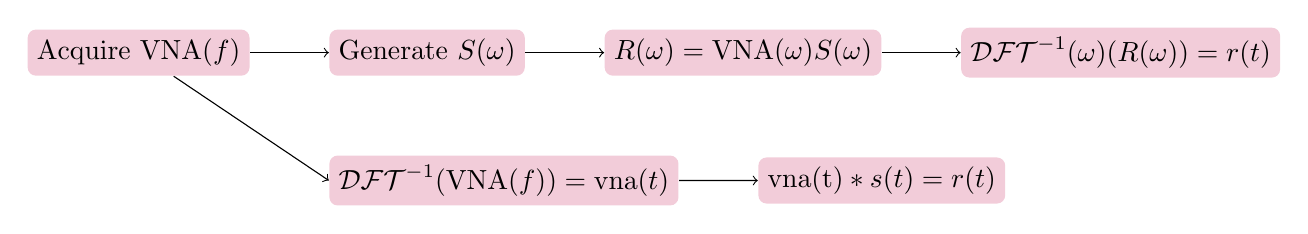
\begin{tikzpicture}
    [scale=.8,auto=left,every node/.style={rectangle,fill=purple!20,rounded
    corners=3pt}]
    % upper branch
    \node (a) at (0,0) {Acquire $ \textrm{VNA}(f) $};
    \node (b) [right=of a] {Generate $S(\omega)$};
    \node (c) [right=of b] {$R(\omega) = \textrm{VNA}(\omega)S(\omega)$};
    \node (d) [right=of c] {$\mathcal{DFT}^{-1}(\omega)(R(\omega)) = r(t)$};
    \draw[->] (a) -- (b); \draw[->] (b) -- (c); \draw[->] (c) -- (d);
    % Lower branch
    \node (e) [below right=of a] {$ \mathcal{DFT}^{-1}(\textrm{VNA}(f)) =
      \textrm{vna}(t) $};
    \node (f) [right=of e] {$ \textrm{vna(t)} * s(t) = r(t)$};
    \draw[->] (a) -- (e.west); \draw[->] (e) -- (f);
  \end{tikzpicture}
  \caption{Workflow for approach 1.}
  \label{fig:approach_1_graph}
\end{figure}

\subsubsection{Caveats: Approach 1}
\label{sub:caveats_approach_1}

\begin{enumerate}
  \item VNA data is assumed to be periodic, but $ S(\omega) $ is not periodic
    ($\mathcal{F}$).
  \item Time-domain points (spacing, number) are constrained by the frequency-domain points.
\end{enumerate}

\subsection{Phillip Dunsmore's Approach - [pdunsmore]}
\label{sub:phillip_dunsmore_s_approach_pdunsmore_}

Phillip Dunsmore's thesis provides a mathematical framework for approaching this
problem. His solution most differs from the na\"{i}ve solution in that the VNA
data is assumed to have been acquired as if a sampling function was applied to
the frequency domain. He uses the sampling function $\Sh(f)$ to pluck off
frequency components. He accounts for the finite frequency domain by applying a
rectangular filter function $\Theta(f_{max})$ to the measured data.

Concretely,

\begin{enumerate}
  \item
\end{enumerate}

\end{document}
